\section{History of Christendom}

\begin{wrapfigure}{rt}{.3\textwidth}
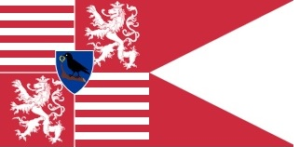
\includegraphics[width=.3\textwidth]{HBanner-300x147.png}
\end{wrapfigure}

\begin{quotationx}
I received this post from an anonymous source. Given the contemporary uncertainty about the notion of ``Identity'' today, and the way it is being played out in Hungary, I decided to post this.

The note that accompanied it indicated that this was written in response to a recent article on the search for the ``real'' Hungarian identity. That article tried to trace back Hungarian identity to some Turanian source. Insofar as Turanian means the Turkish peoples across Asia, there may be a point. However, it seems to include Orientals such as the Mongols and even the Japanese. Moreover, that same web site has another talk that claims the Turanians were actually Persians.

So which is it? Are current Hungarians misplaced Turks in the heart of Europe, or are they ultimately descendants of Hyperborea through the Persian line? And, in the best case, even if the truth be known, what does it really say about Hungarian identity?

Man is a spiritual being, so his real identity is the spiritual impulse of a people. This is manifested in the social and political life of a people. Genetics come last: they are a creation of the Spirit, not the other way around. So this post demonstrates that the spiritual impulse behind the Hungarian nation has historically been Catholicism. The impulse is first carried by the great men of a nation and then is given to the people, as illustrated below. In a similar way, France was the creation of 40 Catholic kings, and it ended in the atheistic Terror.

Such leaders understand human nature. People are not motivated by intellectual arguments, but instead by a spiritual vision. Once that vision is lost, the people are in decline. Those who take a strictly Darwinian view of man cannot account for that. What Darwinian principle predicts that a related genetic group would consider it abnormal to protect its boundaries and ways of life? Why do Western governments need to give monetary incentives, or blast the media with propaganda, to convince their populations to have more children?

Nor is the latest intellectual fad a suitable replacement for the life of the spirit. Nations are not motivated in that way. Rationalism cannot account for the surds of concrete existence (as we will show in a future post). An idea may win an election every now and then, but that is no permanent solution. What is lacking is the notion of permanency.
\textbf{Vladimir Solovyov} explains:

\begin{quote}\small

Prior to Christianity, the fixed foundation of life was human nature and the divine was the principle of change, motion, progress. After Christianity, the divine, as incarnate, becomes the fixed foundation, the element of life for humankind.
\end{quote}


When material progress is made the fixed foundation, then decline is inevitable. Solovyov makes this clear:

\begin{quote}\small
Any attempt to make the material principle the sole basis of life would inevitably lead to the disintegration of humankind, to the destruction of society and science, to universal chaos.
\end{quote}


An intellectual argument is hardly necessary at this point; all one need do is to look around with a clear and detached vision. And don't count on chaos magick and matriarchy to find the way out and back. We don't need yet another ``political theory'', but rather the remembrance of our fixed foundation.
\end{quotationx}


\paragraph{Hungary}

\begin{wrapfigure}{rt}{.3\textwidth}
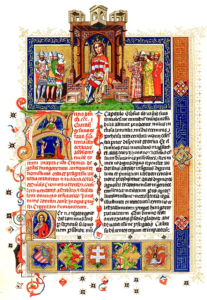
\includegraphics[width=.3\textwidth]{ChronicaHungarorum-207x300.png}
\end{wrapfigure}

\textbf{Chronicon Pictum}. The Chronicon Pictum\footnote{Latin for ``illustrated chronicle''; in English\textbf{: Illuminated Chronicle or Vienna Illuminated Chronicle}; Hungarian: \textbf{Képes Krónika} also referred to as \textbf{Chronica Hungarorum, Chronicon (Hungariae) Pictum, Chronica Picta} or \textbf{Chronica de Gestis Hungarorum}} is a medieval illustrated chronicle from the Kingdom of Hungary from the second half of fourteenth century. It represents the international artistic style of the royal courts in the court of Louis I of Hungary.

Its full name is \emph{Chronicon pictum, Marci de Kalt, Chronica de gestis Hungarorum}, that is, the \emph{Illustrated Chronicle, Mark of Kalt's Chronicle About the Deeds of the Hungarians}.

Written in the year 1358, with the last of the illuminations being finished between 1370 and 1373, the chronicle was given by the Hungarian king Louis I to the French king Charles V when the daughter of Louis, Catherine, was engaged to Charles' son Louis I, Duke of Orléans.

It was then gifted to Dorde Brankovic, titular Despot of Serbia. The title given to him in 1486 by Matthias Corvinus whoruled a region known as Racszag (after Rascia, being equivalent of modern Vojvodina) under the Kingdom of Hungary. In 1456, where it was copied, and later lost, possibly spending some time in Turkish possession.

The chronicle reappears in the first half of the 17th century in the royal archives of Vienna by unknown means. This is why it is also referred as the \emph{Vienna Illuminated Chronicle}. The manuscript is now kept in the National Szechenyi Library in Budapest (Orszagos Szechenyi Konyvtar, Budapest).

The 147 pictures of the chronicle are a great source of information on medieval Hungarian cultural history, costume, and court life in the 14th century. Many miniatures seen inside this chronicle are painted with gold. The artistic value of the miniatures is quite high, if we compare similar miniatures from other parts of Western Europe from the same time. The characters are drawn with detail and with knowledge of anatomy. Even the eyeballs are painted, which can only be checked through microscope. Such refinement and ``hoch style'' speak of a great attentiveness and care in producing these marvels, as well as already then expressed nation's honour of tradition and history and the pride in their common Christian religion. All miniatures showing Attila the Hun are disrupted or even rubbed out (especially the last, showing Attila's death); this cannot be due to the time as all other miniatures and text are preserved well. So we conclude that it must have been done on purpose.

\begin{wrapfigure}{rt}{.3\textwidth}
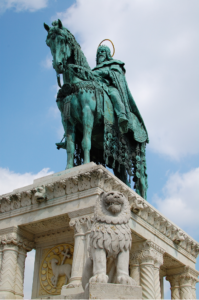
\includegraphics[width=.3\textwidth]{SaintStephen-199x300.png}
\end{wrapfigure}

This is the text version for our respected Hungarian readers Képes Krónika\footnote{\url{http://mek.oszk.hu/10600/10642/10642.htm\%20target=}} and this one for Gentlemen versed in Latin: Chronicon Budense\footnote{\url{https://books.google.hr/books?id=s4wAAAAAcAAJ&pg=PR1&redir\_esc=y\#v=onepage&q&f=false}} .

Link to a version of Chronica Hungarorum (1488, Theobald Feger, Erhard Ratdolt. Augsburg, Pergamen) : Chronica Hungarorum\footnote{\url{http://www.corvina.oszk.hu/corvinas-html/hub1inc1143.htm}}.

\paragraph{Hungarian Principality}

\textbf{Magyar Nagyfejedelemseg}: The ``Hungarian Grand Principality,'' Duchy of Hungary was established in 895 or 896, due to the Hungarian conquest of the Carpatian basin, a series of historical events ending with the settlement of the Hungarians in Central Europe at the turn of the 9th and 10th centuries. They gradually settled in the Basin and established a Christian monarchy, the Kingdom of Hungary around 1000, with the coronation of Saint Stephen, until 1918, when Charles IV ``renounced participation'' in state affairs but did not abdicate. The Arpad dynasty, the male-line descendants of Grand Prince Arpad, ruled Hungary continuously from 895 to 1301.

\textbf{Szent István Kiraly}\footnote{some interesting disambiguation for the interests in the naval force and strategy Szent István\footnote{\url{https://en.wikipedia.org/wiki/SMS\_Szent\_István}}; Latin: Sanctus Stephanus} was the last Grand Prince of the Hungarians between 997 and 1000 or 1001, and the first King of Hungary from 1000 or 1001 until his death in 1038. He was crowned on 25 December 1000 with a crown sent by \textbf{Pope Sylvester II}.

\textbf{Crowning}. Thietmar of Merseburg writes that Stephen received the crown ``with the favour and urging'' of \textbf{Emperor Otto III} (r. 996--1002) --- Holy Roman Emperor of the Ottonian dynasty (Ottonian dynasty\footnote{\url{https://en.wikipedia.org/wiki/Ottonian\_dynasty}}) --- implying that Stephen accepted the Emperor's suzerainty before his coronation. On the other hand, all of Stephen's legends emphasize that he received his crown from Pope Sylvester II (r. 999--1003). Kristo and other historians point out that Pope Sylvester and Emperor Otto were close allies, which implies that both reports are valid: Stephen ``received the crown and consecration'' from the Pope, but not without the Emperor's consent. Around 75 years after the coronation, Pope Gregory VII (r. 1075--1085), who claimed suzerainty over Hungary, declared that Stephen had ``offered and devotedly surrendered'' Hungary ``to Saint Peter'' (that is to the Holy See). Another report, Stephen's Greater Legend, states that the King offered Hungary to the Virgin Mary.

\textbf{Spreading Christianity}. Stephen established at least one archbishopric, six bishoprics and three Benedictine monasteries; thus the Church in Hungary developed independently of the archbishops of the Holy Roman Empire. He encouraged the spread of Christianity with severe punishments for ignoring Christian customs. His system of local administration was based on counties organized around fortresses and administered by royal officials. Hungary, which enjoyed a lasting period of peace during his reign, became a preferred route for pilgrims and merchants traveling between Western Europe and the \textbf{Holy Land or Constantinople}.

He died on 15 August 1038 and was buried in his new basilica, built in Szekesfehervar and dedicated to the Holy Virgin. His death caused civil wars which lasted for decades. He was canonized by Pope Gregory VII, together with his son, Emeric, and Bishop Gerard of Csanad, in 1083. Stephen is a popular saint in Hungary and the neighbouring territories. In Hungary, his feast day (celebrated on 20 August) is also a public holiday commemorating \textbf{the foundation of the state}.

\textbf{Andrew I the White} or the Catholic\footnote{Hungarian: I. Feher or Katolikus Andras or Endre; c. 1015 -- Zirc, before 6 December 1060.} was King of Hungary from 1046 to 1060. He descended from a younger branch of the Arpad dynasty. After spending fifteen years in exile, he ascended the throne during an extensive revolt of the pagan Hungarians. He strengthened the position of Christianity in the Kingdom of Hungary. Before his coronation a revolt had broken out in Hungary that was dominated by pagans who captured many clergymen and mercilessly slaughtered them.

Most Hungarian lords and the prelates opposed the restoration of paganism. They preferred the devout Christian Andrew to his pagan brother Levente. The Hungarian chronicles write that Levente, who died in short time, did not oppose his brother's ascension to the throne. Historian Ferenc Makk writes that Andrew was crowned with a crown that the Byzantine Emperor Constantine IX Monomachos had sent to him. Nine enamelled plaques from this golden crown were unearthed in Nyitraivánka (Ivanka pri Nitre, Slovakia) in the 19th century.

\begin{quotex}
Having now been made secure against all disturbances from enemies, Duke Andreas received the crown of kingship in the royal city of Alba. No more than three bishops who had escaped that great slaughter of the Christians performed the ceremony of coronation in the year of our Lord 1047. He made proclamation to all his people that under pain of death they should lay aside the pagan rites which had formerly been permitted to them, and that they should return to the true faith of Christ and live in all things according to the law which King St Stephen had taught them.
\flright{\textit{The Hungarian Illuminated Chronicle}}
\end{quotex}


Andrew's wife, Anastasia, was the daughter of Grand Duke Yaroslav I the Wise of Kiev by his wife, Ingegerd, who herself was the daughter of King Olof Skotkonung of Sweden.

\paragraph{Second Founder of the State}


Bela IV (1206 -- 3 May 1270) was King of Hungary and Croatia between 1235 and 1270, and Duke of Styria from 1254 to 1258. Bela was appointed Duke of Slavonia, also with jurisdiction in Croatia and Dalmatia. Around the same time, Bela married Maria, a daughter of Theodore I Laskaris, Emperor of Nicaea. From 1226, he governed Transylvania with the title Duke. He supported Christian missions among the pagan Cumans who dwelled in the plains to the east of his province. Some Cuman chieftains acknowledged his suzerainty, and he adopted the title of King of Cumania in 1233.

\textbf{The Mongols invaded Hungary} and annihilated Bela's army in the Battle of Mohi on 11 April 1241. He escaped from the battlefield, but a Mongol detachment chased him from town to town as far as Trogir on the coast of the Adriatic Sea. Although he survived the invasion, the \textbf{Mongols devastated the country} before their unexpected withdrawal in March 1242. Bela introduced radical reforms in order to prepare his kingdom for a second Mongol invasion. He allowed the barons and the prelates to erect stone fortresses and to set up their private armed forces. He promoted the development of fortified towns. During his reign, thousands of colonists arrived from the Holy Roman Empire, Poland, and other neighbouring regions to settle in the depopulated lands. Bela's efforts to rebuild his devastated country won him the epithet of ``second founder of the state'' (Hungarian: \textbf{Masodik honalapito}).

He set up a defensive alliance against the Mongols, which included \textbf{Daniil Romanovich, Prince of Halych, Boleslaw the Chaste, Duke of Cracow and other Ruthenian and Polish princes.} His allies supported him in occupying the Duchy of Styria in 1254, but it was lost to King Ottokar II of Bohemia six years later. During Bela's reign,\textbf{a wide buffer zone}---which \textbf{included Bosnia, Barancs (Branicevo}, \textbf{Serbia}) and other newly conquered regions---was established along the southern frontier of Hungary in the 1250s.

\paragraph{Sigismund of Luxembourg.}


\emph{Saving of the Constantinople. ``O Quam Misericors est Deus, Pius et Justus''.}

Sigismund of Luxembourg (15 February 1368 in Nuremberg -- 9 December 1437 in Znaim, Moravia) was Prince-elector of Brandenburg from 1378 until 1388 and from 1411 until 1415, King of Hungary and Croatia from 1387, King of Germany from 1411, King of Bohemia from 1419, King of Italy from 1431, and \textbf{Holy Roman Emperor} for four years from 1433 until 1437, the last male member of the House of Luxembourg. Sigismund von Luxembourg was the leader of the last Western European Crusade --- the Crusade of Nicopolis of 1396 to liberate Bulgaria and save Constantinople from the Turks. By his initiative and key role, the \textbf{Council of Constance (1414--1418)} was summoned to resolve the Western---also known as the Papal---Schism. After the victory at Dobor, he established monarchical chivalric order with the sole purpose to fight Turks. All major Royal Houses became members of the Societas Draconistarum. Sigismund was inspired by the order of Saint George of as well as the Sicilian Order of the Ship, founded in 1381. After \textbf{the Fall of Constantinople} in 1453, it continued to play a role in Hungary, Croatia, Serbia, and Romania, which bore the heavy burden of the Ottoman incursions.

It would take several tomes to write about each Hungarian King to the extent we would want to, as many of them are champions amongst the Princes in Christendom. We have chosen the four previously mentioned to show the principle, which is our Cross and \textbf{Viribus Unitis}.

\textbf{Österreichisch-Ungarische Monarchie, Osztrak-Magyar Monarchia. Indivisibiliter ac Inseparabiliter.} Austria--Hungary was a constitutional union of the Austrian Empire (the Kingdoms and Lands represented in the Imperial Council, or Cisleithania) and the Kingdom of Hungary (Lands of the Crown of Saint Stephen or Transleithania) that existed from 1867 to 1918, when it collapsed as a result of defeat in World War I. The union was a result of the Austro-Hungarian Compromise of 1867 and came into existence on 30 March 1867. Austria-Hungary consisted of two monarchies (Austria and Hungary) and one autonomous region, the Kingdom of Croatia-Slavonia under the Hungarian crown, which negotiated the Croatian--Hungarian Settlement (Nagodba) in 1868. It was ruled by the House of Habsburg and constituted the last phase in the constitutional evolution of the Habsburg Monarchy. Following the 1867 reforms, the Austrian and the Hungarian states were co-equal. Foreign affairs and the military came under joint oversight, but all other governmental faculties were divided between respective states.

\paragraph{Religion in Hungary}


\textbf{International Social Survey Programme} 2015 found that 83.4\% of the Hungarian population declared to belong to a Christian denomination, with Catholicism being the largest denomination amounting to 62.6\% of the respondents (including Greek Catholics at 3.2\%), Calvinism was the second-largest sect amounting to 16.6\%, and Lutheranism the third-largest with 3.2\%. A further 15.5\% declared to have no religion, 1.0\% to belong to another Christian denomination and 0.9\% declared to belong to other religions.

In 2018, according to a study jointly conducted by London's St Mary's University's Benedict XVI Centre for Religion and Society and the Institut Catholique de Paris, and based on data from the European Social Survey 2014--2016, among the 16 to 29 years-old Hungarians 33\% were Christians (26\% Catholic, 6\% Protestant and 1\% other Christians) and 67\% were not religious. In long term this might be a near future problem for Hungary which is facing the paneuropean problem of immigration, effluence of religion, as well as the devastating influence of modern philosophical currents --- which through time and neglect will even more deteriorate the true European spirit that has been christened for over 1000 years in an unbroken tradition: a spiritual tradition which is a true golden binding in the manifold Being of the life of a people --- as ethnos, as social unity, as a State. Such spiritual tradition is diametrically opposite to the Turanian notions and perfidious suggestibility of this article, for example: TIBOR IMRE BARANYI: WHO IS THE ENEMY OF HUNGARIAN IDENTITY?\footnote{\url{https://www.geopolitica.ru/en/article/tibor-imre-baranyi-who-enemy-hungarian-identity}}.


\flrightit{Posted on 2018-08-06 by Anonymous}

\begin{center}* * *\end{center}

\begin{footnotesize}
\begin{sffamily}
\texttt{Max on 2018-08-09 at 18:33 said:}

Replying to the article linked to above; Christianity may appear to be dead... Mohammedanism however, appears to be living. How comforting that your neighbour is an animated corpse, whose main concern now seems to be that it is confused about its identity. ``Why they go to the West in the first place?'' That is the question. Assuredly not from a state of inner health. According to ancient mythology, the West is the region of the dead. It is simple really: They come here to die. We have navigated these waters for a long time already, and it has taken a toll, with the interior lifelessness and all. It is a struggle, but listen and you might yet live.

To believe that human life and spiritual realities are fundamentally conditioned by geography, as in ``geopolitics'', is just another variant of dialectical materialism. In dystopic novels we are introduced the notion of a war between the continents, on seemingly no other pretext than disassociated and accidental physical occupation. The Russian-flavored globalist psyops peddling ``geopolitics'' ``multipolarity'' ``atlanticism'' ``eurasianism'' and so forth plays precisely into this scenario.

Useful idiots suddenly becomes all eager to offer geopolitical analyses on every little trifle, instead of concerning themselves with what is of value closer to home. Lines and figures drawn on a map does not have consciousness or intent -- humans with all that motivates them do. Now, to be primarily motivated by the map is part of the problem and not the solution.

These people honestly seem to think that the movement they term ``globalism'' is restricted to a confined region of the globe, while the weakening of American dominance was part of the game all along.

Concerning the ravings about ``atlanticism'', we are certainly well aware of the Mongols deep seated fear of water -- they did after all do the opposite of going to the ends of the world in order to settle as far away form it as possible -- but it is simply nonsensical to make an elemental fear into a modern myth governing political action. The material conditions of a land mass does not create spirit.

Furthermore, if Russia according to a ``geopolitical'' strategy were to expand to include more coastal borders, it would thereby, according to its own doctrine, become an evil atlanticist power itself. Just spare us the drama and idiocity and retreat back into central asia.

\hfill

\texttt{Max on 2018-08-30 at 15:17 said:}

Not many places seem to mention that ``1984'' is likely an allusion to a hypothethical ``hundred-year-plan'' counting from the foundation of the Fabian society in 1884. Bolsheviki five-year-plans are only meant for the duped proletariat. Judging by the circumstances, that book must have been more or less directly commisioned by the same people who also provided the means to write it.

Art is often more truthful and accurate than the output of academics. Continuing on the same theme, another novel came to attention, which although I have not read it yet, demonstrates a foresight that must be difficult to neglect. In an academic paper, Piper describes the plot of St Peter's Snow:

``The Baron's plan was `to rekindle the glow of faith in an age that has grown tepid and empty' and `to lead the hearts of mankind back to the glamour of the throne and the idea of empire by the grace of God.' The idea is rejected in a discussion with the local priest, who believes that `faith is a blessing (that) can only be kindled by patient work, by loving science, and by prayer,' but the Baron's scientific assistant Kallisto says `No, it can also be kindled by chemistry.''

The scientists supposedly sought to synthesize the substance that they speculated were in use in the Eleusinian mysteries in order to inaugurate a religious revival and restore the Holy Roman Empire, although the twist is that the subsequent ``awakening'' instead turns into a communist revolution.

Eliade in his well known ``Shamanism'' records how the use of psychoactives is a symptom of the shaman having lost his power, and more or less have to resort to faking it during the final, much corrupted, stages of the tradition in question. During modern times, corrupt remnants were studied by the counter-tradition as methods to manipulate the population in manufactured states of heightened suggestibility.

\hfill

\texttt{Anonymus on 2018-08-30 at 21:22 said:}

Thank you for your comments.


\hfill

\end{sffamily}
\end{footnotesize}

